\chapter{绪\hspace{6pt}论}
\label{chapter:introduction}

\section{研究工作的背景与意义}
\label{sec:intro}
\subsection{研究背景}
\label{subsec:intro-background}

随着信息技术产业的高速发展,数字信息量呈爆炸式增长。国际数据资讯公司(IDC)\citing{IDC}于2020年公布的统计及预测报告\citing{DataReport2020}显示,每年新产生的数据量在2015年至2025年间以约26\%的复合年增长率增长,预计仅2025年创建的新数的据数据量就将高达175.8\,ZB(而在2015年时仅为18.2\,ZB)。新创建数据量的快速增长导致个人及企业面临的数据存储和管理成本快速上涨\citing{敖莉2010重复数据删除技术}。与此同时,各类型数据中存在不同程度的冗余缩减空间。平均而言,各类型数据存储系统具有逾60\%的冗余缩减机会。并且,随着存储系统的持续运行,冗余数据占比逐步上升\citing{mcknight2006digital}。利用存储系统内数据冗余度高的特点来节省存储空间、降低存储管理开销成为热门研究课题。

重复数据删除(Data deduplication)\citing{付印金2012重复数据删除关键技术研究进展, 敖莉2010重复数据删除技术,xia2016Deduplication,Paulo2014}是一种粗粒度的数据冗余缩减技术。传统数据压缩针对小规模数据(例如,同一文件内部),使用字节级重新编码以降低冗余;作为对比的,重复数据删除以数据块(大小通常为8\,KiB)为基本单位缩减冗余,其通过比较来自相同和不同文件的数据块,为具有相同内容的数据块仅保存一份物理拷贝以节约存储空间。如图~\ref{fig:Deduplication-storage-pattern}所示,在支持重复数据删除的各类存储系统(统称为重复数据删除系统)中,重复数据删除后的任何数据块都被一个或多个文件引用,而每个文件则以指向这些数据块的指针的集合形式进行存储。重复数据删除可为主存和备份数据分别节省50\%\citing{meyer2011deduplication}和98\%\citing{wallace12}的存储空间,可显著降低云存储厂商及个人的存储维护成本\citing{付印金2012重复数据删除关键技术研究进展}。由于能够有效地降低存储开销,重复数据删除技术非常适合为管理日益增长的海量数据节省成本。在工业界,Dell EMC Data Domain\citing{EMCDataDomain}、Avamar\citing{Avamar}、Veritas的NetBackup Appliances\citing{veritas}以及Commvault的开放数据平台\citing{CommVault}都是较为知名的重复数据删除应用产品。此外,各大云存储厂商(例如:Dropbox\citing{Dropbox}、Google Drive\citing{GoogleDrive}、百度网盘\citing{BaiduPan}等)也纷纷将重复数据删除技术应用于各自的云存储产品中,以提升经济效益\citing{harnik2010side}。

\begin{figure}[!htb]
  \small
  \centering
  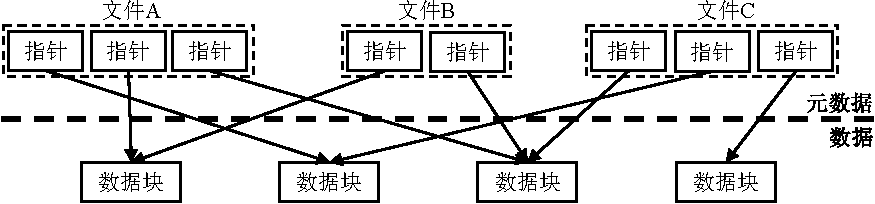
\includegraphics[width=\textwidth]{pic/background/dedupOverview.pdf}
  \caption{重复数据删除系统的存储模式}
  \label{fig:Deduplication-storage-pattern}
\end{figure}

\textbf{本文重点关注面向云环境的重复数据删除。}图~\ref{fig:Cloud-based-deduplication-storage-logic}描述了基于源端重复数据删除\textit{(Source-based deduplication)}构建的云环境重复数据删除系统框架。云服务商维护哈希索引表,记录所有已存储数据块的哈希值;在重复数据删除过程中,用户使用云存储客户端计算目标数据块的哈希值;云服务商检查该哈希值是否存在于数据块索引表中,如果哈希值存在(即云服务端已有目标数据块的副本),则更新目标数据块的所有权信息并通知客户端无需传输该数据块,从而同时节省传输带宽和存储空间。然而,由于重复数据删除系统中任意重复数据块均只保留一个副本,任意一个数据块的泄露产生的影响可能扩散共用该数据块的所有文件。这种文件共用数据块的存储模式强调了数据块的敏感性。因此,如何保护重复数据删除后的数据的隐私,成为云存储服务商应用重复数据删除技术时亟需解决的关键问题。

\begin{figure}[!htb]
  \small
  \centering
  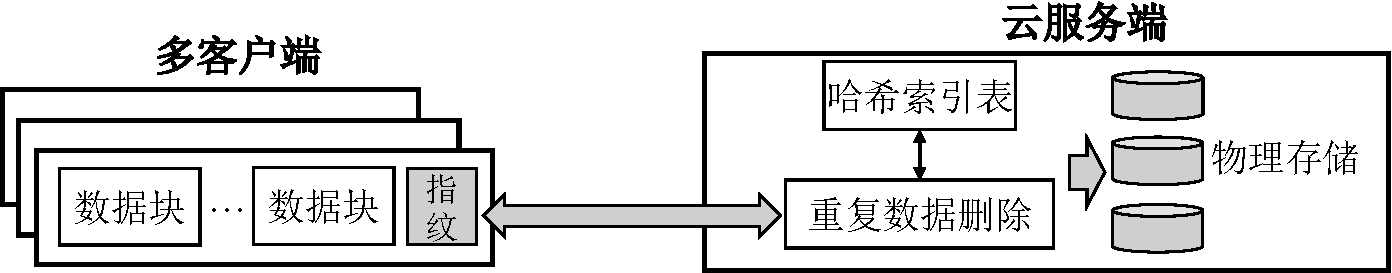
\includegraphics[width=\textwidth]{pic/background/Cloud-deduplication.pdf}
  \caption{云环境重复数据删除系统结构}
  \label{fig:Cloud-based-deduplication-storage-logic}
\end{figure}
%TODO
近年来,研究者提出加密后重复数据删除\citing{bellare2013MLE}以保护重复数据删除过程中的数据安全。图~\ref{fig:Cloud-based-encrypted-deduplication-storage-logic}描述了加密后重复数据删除系统框架,其包括客户端和云服务端两个主要组成部分。为了防止云服务商获取外包数据内容,加密后重复数据删除系统在客户端部署消息锁加密\textit{(Message-locked encryption, MLE)}\citing{bellare2013MLE}以加密明文数据块(简称为明文数据块),同时确保重复数据删除仍然能够作用于密文数据块(简称为密文数据块)以节约存储空间。传统对称加密算法为每个客户端或每个数据块分配不同加密密钥,使得相同的明文数据块被加密为不同的密文数据块,无法通过重复数据删除进行冗余消除。消息锁加密的核心思路是基于数据块内容产生密钥(称为MLE密钥,例如基于明文数据块的哈希值\citing{douceur2002reclaiming}产生),从而实现明文数据块和密文数据块的一一映射。最终,实现具有等同冗余缩减能力的直接针对密文数据块的重复数据删除。现有消息锁加密采用服务器辅助密钥生成方式(称为服务器辅助消息锁加密\textit{(Server-aided MLE)}\citing{bellare2013DupLESS}),即部署第三方密钥服务器管理全局秘密,同时基于明文数据块哈希值和密钥服务器的全局秘密共同生成消息锁加密密钥,以防止攻击者针对MLE密钥实施离线暴力破解攻击。

\begin{figure}[!htb]
  \small
  \centering
  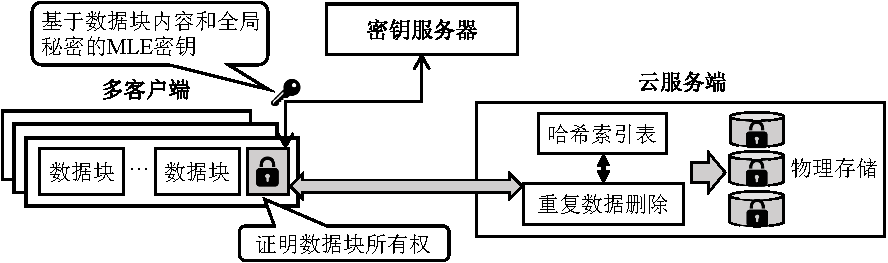
\includegraphics[width=\textwidth]{pic/background/Cloud-encrypted-deduplication-logic.pdf}
  \caption{面向云环境的加密后重复数据删除系统框架}
  \label{fig:Cloud-based-encrypted-deduplication-storage-logic}
\end{figure}

另一方面,重复数据删除受到伪造数据所有权的攻击威胁\citing{harnik2010side,mulazzani11}。由于云服务商仅基于收到的数据块哈希值判断客户端是否拥有相应数据块,恶意用户/客户端可以伪造任意密文数据块的哈希值,如果该密文数据块已在云服务端存储(即已发生重复数据删除),则恶意客户端无需传输密文数据块内容便可获得相应密文数据块的访问权限。为了防止伪造所有权攻击,加密后重复数据删除增加了所有权证明\textit{(Proof-of-Ownership)}技术\citing{halevi11}:除了密文数据块的哈希值以外,云服务商要求客户端额外提交目标密文数据块的所有权证明\textit{(Proof)};云服务商首先基于证明验证该客户端是否真实且完整拥有相应密文数据块,然后再执行如前所述的重复数据删除过程。所有权证明技术的合理性在于,只针对客户端真实拥有(即具有完整访问权限)的密文数据块执行重复数据删除,从而避免非法访问其他客户端已在云服务端存储的内容。

\subsection{问题和动机}
\label{subsec:intro-problem}

现有面向云环境的加密后重复数据删除系统面临着系统效率低与安全性不足的双重挑战:

\subsubsection{系统效率}
\label{subsubsec:intro-problem-performance}

在服务器辅助密钥生成过程中,现有加密后重复数据删除系统(图~\ref{fig:Cloud-based-encrypted-deduplication-storage-logic})须使用基于盲签名\citing{armknecht2015transparent,bellare2013DupLESS}的无记忆伪随机函数\textit{(Oblivious pseudorandom function, OPRF)}生成密钥\citing{bellare2013DupLESS},以防止密钥服务器获得明文数据块的哈希值。同时,为了实现所有权证明,系统须在云服务端维护Merkle哈希树,并基于哈希树验证客户端提交的证明信息\citing{halevi2011proofs}。本文指出,服务器辅助密钥生成和所有权证明的密码操作是加密后重复数据删除系统的主要效率瓶颈。

为了验证以上论断,本文基于图~\ref{fig:Cloud-based-encrypted-deduplication-storage-logic}框架和现有技术方案实现了加密后重复数据删除系统的基础原型。基础原型支持基于RSA\citing{bellare2013DupLESS}或BLS\citing{armknecht2015transparent}盲签名生成密钥,以及基于Merkle哈希树\citing{halevi2011proofs}或通用哈希\textit{(Universal hash)}\citing{xu2013weak}证明所有权(注:基于通用哈希的所有权证明方法\citing{xu2013weak}只能达到较低安全性)。

\begin{table}[!htb]
  \small
  \centering
  \begin{tabular}{@{}ccc@{}}
    \toprule
                                & 处理阶段/可选方案            & 处理时间(ms/MiB) \\ \midrule
                                & 数据分块                     & 3.8              \\
    服务器辅助密钥生成          & RSA盲签名方案(BLS盲签名方案) & 40.7(488.3)      \\
    \multirow{3}{*}{所有权证明} & 数据加密                     & 2.5              \\
                                & 哈希树方案(通用哈希方案)     & 27.0(7.2)        \\
                                & 重复数据删除                 & 1.7              \\ \bottomrule
  \end{tabular}
  \caption{基础原型每个步骤处理1MiB数据的时间开销:括号内为可供备选的服务器辅助密钥生成方案和所有权证明方案,以及相应处理时间}
  \label{tab:intro-bottleneck}
\end{table}

表~\ref{tab:intro-bottleneck}展示了基础原型每个步骤处理1MiB数据的平均时间开销。服务器辅助密钥生成是最大效率瓶颈。如果采用基于Merkle哈希树的所有权证明方案,RSA盲签名和BLS盲签名分别占系统总开销的53.8\%和93.3\%。同时,所有权证明也是限制系统效率的重要因素,如果采用基于RSA盲签名的服务器辅助密钥生成方案,Merkle哈希树和(较低安全性的)通用哈希方案分别占系统总开销的35.7\%和9.5\%。

\subsubsection{安全隐患}
\label{subsubsec:intro-problem-security}

现有支持数据块所有权证明技术的加密后重复数据删除依然不足以完全击败恶意客户端。在重复数据删除过程中,云服务商通知客户端传输或不传输密文数据块内容(\S\ref{subsec:intro-background}) ,实质上泄漏了“其他客户端是否已经存储相应密文数据块”的侧信道信息\textit{(Side-channel information)}。虽然所有权证明阻止了针对非授权密文数据块的重复数据删除,但不足以防止恶意客户端的侧信道攻击。例如,攻击者可以枚举所有可能的数据内容,并利用重复数据删除泄漏的侧信道信息实施推测内容攻击(\textit{Learning-content attack})\citing{harnik2010side,zuo2018mitigating}。假设攻击者已知某个客户端持有目标文件且文件内容符合固定的公开格式(例如工资条、合同等模版化数据),致力于推断目标文件未公开的敏感内容(例如薪水金额)。攻击者枚举所有可能的未公开内容,并通过恶意客户端上传所生成的枚举文件。如果上传某个枚举文件时无需传输任何密文数据块,即可推断该枚举文件即为目标文件。此时,由于攻击者完全获得了所枚举文件的访问权限,仅检测所有权无法阻止推测内容攻击。

\subsection{研究内容概述}
\label{subsec:intro-content}

本文指出,现有加密后重复数据删除使用纯软件实现的密码算法保障数据安全,但是,由于密码算法计算开销大、安全防护不完整,导致当前的重复数据删除系统存在效率和安全方面的不足。因此,本文拟开展基于硬件可信执行环境的安全重复数据删除研究,意图通过硬件实现的可信执行环境\textit{(Trusted execution environment, TEE)}优化/改变现有基于纯软件的重复数据删除方法思路,进而克服现有研究的不足。具体的,TEE是一组软硬件结合的系统组件,可为应用程序提供必要的基础设施和运行资源,同时为内部代码的安全执行提供机密性和完整性保证\citing{OMTP}。各大软硬件厂商均推出了各自的TEE实现方案,包括TrustZone\citing{trustzone}、Intel SGX\citing{sgx,sgx2}、AMD SEV\citing{AMDSEV}、Apple Secure Enclave\citing{AppleSecureEnclave}、Google Titan\citing{GoogleTitan}等。为了避免硬件依赖,本文的系统设计并不基于某一具体的TEE解决方案,统一使用“安全区”指代TEE实现的具有隔离条件和安全保障的程序执行环境。本文的核心方法是,在安全区内执行面向明文数据的敏感操作,以基于硬件的保护方式替代传统基于纯软件实现的复杂密码算法,从而保持安全性并提高系统效率。

针对现有面向云环境的加密后重复数据删除存在密钥生成效率低、所有权证明计算复杂、易于遭受推测内容攻击等不足。本文拟改进现有的加密后重复数据删除方法,提出:

\begin{enumerate}[leftmargin=0em]
  \item 基于TEE的轻量级密钥生成技术,以提升服务器辅助密钥生成的效率。
  \item 基于TEE的高效所有权证明技术,以提升数据所有权证明效率。
  \item 基于TEE的扩展所有权证明技术,以进一步防止推测内容攻击(现有所有权证明技术不足以防止推测内容攻击,见\S\ref{subsubsec:intro-problem-security})。
\end{enumerate}

\subsection{研究意义}
\label{subsec:intro-meaning}

在学术界,自收敛加密\citing{douceur2002reclaiming}提出以来,安全重复数据删除已有20余年研究历史,但由于一些本质问题(例如效率、侧信道攻击、密钥管理等,见\S\ref{subsec:intro-problem})未能得到妥善解决而难以落地推广;并且,目前的学术研究聚焦于解决某一方面本质问题,同时以牺牲另一方面性能为代价(\S\ref{subsubsec:intro-problem-performance})。本文的学术研究意义在于,\textbf{突破现有安全重复数据删除方法局限,同时妥善解决效率、安全、存储多个本质问题,推动安全重复数据删除理论到实践的转化。并且,本文作为TEE在数据存储领域的应用范例,所提出的系统和方法对TEE在其他领域研究具有参考价值。}

在工业界,本文研究的安全、效率、成本问题是云服务商关注的焦点问题。一方面,数据安全隐私和服务使用体验,是决定用户是否选择云服务的关键因素;另一方面,重复数据删除有助于降低设备购置和维护成本,提升云服务商的经济效益。因此,本文的应用实践价值在于,\textbf{在云服务商关注的安全、效率、成本维度,研究的系统和方法将全面领先于现有基于纯软件的安全存储解决方案,将推动未来基于TEE的云存储架构,对促进云服务产业发展具有积极意义。}

\section{国内外研究历史与现状}
\label{sec:compare}

\subsection{加密后重复数据删除}
\label{subsec:compare-deduplication}

\S\ref{subsec:intro-problem}指出了加密后重复数据删除系统面临的系统效率、安全隐患方面的不足,接下来将综述现有的针对性解决方法及其与本文研究内容的区别。

\subsubsection{系统效率}
\label{subsubsec:compare-deduplication-performance}

为了解决服务器辅助密钥生成效率瓶颈,SecDep\citing{zhou2015secdep}提出生成粗粒度的文件级MLE密钥,并针对不同用户之间的相同数据使用文件级重复数据删除;本文提出了基于相似性密钥生成方法\citing{qin17},为若干个连续明文数据块生成基于代表性明文数据块(例如其中具有最小哈希值的明文数据块)的MLE密钥,用以加密其中的每个明文数据块。以上方法均是通过减少MLE密钥生成次数来解决效率问题,但导致部分相同的明文数据块被加密为不同的密文数据块而无法被删除。本文研究的基于TEE的轻量级密钥生成技术将提升单次密钥生成速率,同时允许删除所有数据块级冗余;研究的加密前重复数据删除方法无需通过服务器辅助方式生成密钥。
在所有权证明方面,研究者通过降低安全性提升效率\citing{xu2013weak,pietro12},但是,本文研究的基于TEE的扩展所有权证明技术将同时提升所有权证明的安全性和效率。

\subsubsection{安全隐患}
\label{subsubsec:compare-deduplication-security}

本文总结分析以下几种可防御推测内容攻击的重复数据删除方案,这些方案均可保护源端重复数据删除中可能泄露的重复数据删除信息。

\begin{enumerate}[leftmargin=0em]
  \item \textbf{目标端重复数据删除(Target-based deduplication)}\citing{harnik2010side}强制客户端传输所有密文数据块后在服务端查找并删除重复的密文数据块,使得重复数据删除过程向客户端完全透明。该防御机制可防止推测内容攻击所依赖的重复数据删除结果信息泄露。
  \item \textbf{随机阈值重复数据删除(Randomized-threshold deduplication)}\citing{harnik2010side}为每个密文数据块分配一个随机阈值,如果密文数据块被上传次数超过阈值,则执行源端重复数据删除(\S\ref{subsec:intro-background}),否则执行目标端重复数据删除。在该方案中,云存储服务端为每个已存储数据块采用的阈值完全随机,使得恶意客户端无法确定该数据块已被上传的次数。
  \item \textbf{两阶段重复数据删除(Two-stage deduplication)}\citing{li2015cdstore}针对来自同一客户端的密文块采取源端重复数据删除,而对来自不同客户端的密文块采取目标端重复数据删除。该防御机制的原理是恶意客户端仅能获得其自身所有数据块的重复数据删除信息。
  \item \textbf{随机冗余数据块传输方案(RRCS)}\citing{zuo2018mitigating}工作在文件级别,其通知每个客户端传输上传文件中的多个随机的重复数据块,以及相应的非重复数据块。该防御机制使得攻击者无法在重复和非重复的文件之间区分传输的数据块个数。
\end{enumerate}

以上方法均须传输全部(目标端重复数据删除)或部分(随机阈值重复数据删除,两阶段重复数据删除和随机冗余数据块传输方案)重复数据,增加网络资源和服务端处理开销。本文研究的基于TEE的扩展所有权证明技术兼容源端重复数据删除而无需传输任意重复数据块。

\subsection{基于TEE的安全应用}
\label{subsec:compare-tee}

TrustZone和SGX是目前应用最广泛的TEE解决方案\citing{pinto19}。TrustZone是ARM CPU指令集的安全扩展,主要应用于低功耗移动平台以保护敏感应用程序的执行逻辑\citing{rubinov2016automated}、用户输入口令\citing{ying2018truz},以及监控安全区以外的程序执行\citing{azab2014hypervision}。SGX是Intel CPU指令集的安全监控扩展,已被广泛用于加强不同应用系统的安全性,包括比特币\citing{matetic19BITE}、文件系统\citing{ahmad2018OBLIVIATE,shinde20}、外包数据库\citing{eskandarian19,priebe18,sun21}、键值存储\citing{mishra2018Oblix,bailleu2019SPEICHER,kim2019ShieldStore,bailleu2021Avocado}和数据分析平台\citing{schuster15, zheng2017Opaque, bowe2020ZEXE}等。

TEE已被广泛用于保护存储系统。PESOS\citing{krahn2018PESOS}使用SGX强化对象存储中的访问策略。OBLIVIATE\citing{ahmad2018OBLIVIATE}增强了基于SGX的文件系统对特权侧信道攻击的安全性。EnclaveDB\citing{priebe18}和ObliDB\citing{eskandarian19}基于SGX保护外包数据库免受信息泄露威胁。NEXUS\citing{djoko2019NEXUS}通过SGX对不受信任的云存储启用细粒度的访问控制。在性能方面,Harnik等人\citing{harnik2018SGX}提出了降低基于SGX系统的性能开销的指南。ShieldStore\citing{kim2019ShieldStore}实现特定于应用程序的数据管理以减少安全区内存开销。SPEICHER\citing{bailleu2019SPEICHER}则是一个基于SGX及LSM树(Log-structured merge-tree)\citing{LSMT}的键值存储系统,具有高效的I/O操作能力。\textbf{然而,以上所有研究均未考虑重复数据删除。}

Dang等人\citing{dang2017Privacy}提出了基于代理的加密后重复数据删除协议,用于低网络资源开销的加密后重复数据删除,但这些协议没有解决密钥生成性能开销,也没有实现相关原型系统。SPEED\citing{cui2019SPEED}利用重复数据删除来提高SGX的计算效率,但本文使用安全区提高了加密后重复数据删除的性能。其他研究使用云服务端安全区实现数据块所有权验证\citing{you2020Proofs}和基于文件的加密后重复数据删除\citing{fuhry2020segshare},而本文使用客户端安全区进行有效地数据块所有权证明生成并支持更细粒度的基于数据块的重复数据删除。SeGShare\citing{fuhry2020segshare}在服务端部署安全区实现文件级重复数据删除,但无法删除相似文件中的相同数据块。S2Dedup\citing{miranda2021S2Dedup}在服务端部署安全区以重加密来自不同客户端的密文数据块,并在安全区外执行针对重加密后密文数据块的重复数据删除,但是,由于所有数据块的重复数据删除均需进出安全区,S2Dedup产生了严重的CPU上下文切换开销\textit{(Context-switching overhead)}\citing{weisse2017regaining}。本文研究的基于TEE的加密后重复数据删除技术可实现对TEE的高效利用,相较于明文重复数据删除系统仅产生有限的额外性能开销。

\section{本文的主要贡献与创新}

\begin{enumerate}[leftmargin=0em]
  \item \textbf{系统性研究如何使用TEE改进重复数据删除,为后续TEE应用起到一定启发作用。}
        尽管已有少量工作提出基于TEE的重复数据删除方法,但这些工作或者只支持粗粒度文件级重复数据删除\citing{fuhry2020segshare},或者由于持续访问安全区外索引导致巨大环境切换开销\citing{miranda2021S2Dedup}。本文明确了如何使用TEE改进现有加密后重复数据删除的密钥生成和所有权证明,以及实现对推测内容攻击的防御,并提供系统以论证实用性。本文所提出的系统和方法对TEE在其他领域研究具有参考价值。
  \item \textbf{研发高效实用的加密前和加密后重复数据删除原型系统,推动安全重复数据删除理论到实践的转化。}
        本文研发的原型系统可以有效解决云存储服务商关注的安全、效率、成本控制等核心问题,并全面领先于现有基于纯软件的高效存储解决方案,推动安全重复数据删除落地实践。
\end{enumerate}

\section{本论文的组织结构}
本文共包含以下五个章节,每个章节的构成如下:

第一章:绪论。本章首先介绍了加密重复数据删除的相关研究背景及尚存的问题,以此为基础提出了本文的研究内容并分析了本文研究工作的意义与价值。随后,总结了加密重复数据删除中性能提升及安全性保障相关的研究工作以及可信执行环境给加密重复数据删除中关键问题的解决提供的新思路;接着,阐述了本文针对安全重复数据删除的性能和安全性做出的 主要贡献及相关的创新之处。最后,给出了本文的章节安排。

第二章:相关基础研究。本章首先介绍了安全重复数据删除技术及其底层的重复数据删除逻辑。详细解读了安全性保障中最关键的数据块加密技术及数据所有权证明技术。随后,介绍了可信执行环境(TEE)及其两种普及的可信执行环境Intel SGX和ARM TrustZone。

第三章:基于可信执行环境加速加密后重复数据删除。本章重点分析介绍了加密重复数据删除中由于数据块加密及数据所有权证明导致的严重性能开销问题,并提出了基于TEE的数据块加密密钥生成方法和数据所有权证明方案。通过三项关键设计将TEE与加密重复数据删除进行有机结合,实现了\sysnameS 的原型系统。最终,通过实验分析证明本文提出的方案相较与现有方案可实现显著性能提升(例如,131.9倍密钥生成速率及9.6倍系统吞吐量)。

第四章:基于可信执行环境对推测内容攻击的主动检测。本章详细分析了第三章提出的\sysnameS 无法应对推测内容攻击的安全隐患,提出了基于客户端安全区进行主动检测攻击的解决方案\sysnameF。在此基础上,提出了相似性保留加密(SPE)以实现基于密文数据块的攻击检测,并给出了理论安全性分析。最后,在\sysnameS 的基础上,本文整合\sysnameF 实现了\prototype 原型系统,同时解决了加密重复数据删除中存在的性能、安全性及网络资源开销问题。通过完备的基于合成或真实世界数据集验证了\sysnameF 的攻击检测能力及\prototype 全方位优于现有加密重复数据删除方案的性能和资源节省能力。

第五章:全文总结与展望。本章对本文提出的关于加密重复数据删除中性能和安全性优化方案进行了总结,并给出了本文后续的三个主要研究方向。
